\documentclass{beamer}

\usetheme{Warsaw}
\usepackage{polski}
\usepackage[utf8]{inputenc}
\usepackage{graphicx}
\graphicspath{ {./img/} }


\title{„NoStat” technologia naukowa dla statystyków}
\institute{ {\huge Instytut Statystyki i Demografii} \\
{ \large Zakład Analizy Historii Zdarzeń  i Analiz Wielowymiarowych}}
\author{dr Sebastian Zając}
\date{22.10.2019}

\begin{document}

% strona tytułowa
\frame{\titlepage}


% strona internetowa
\begin{frame}{}
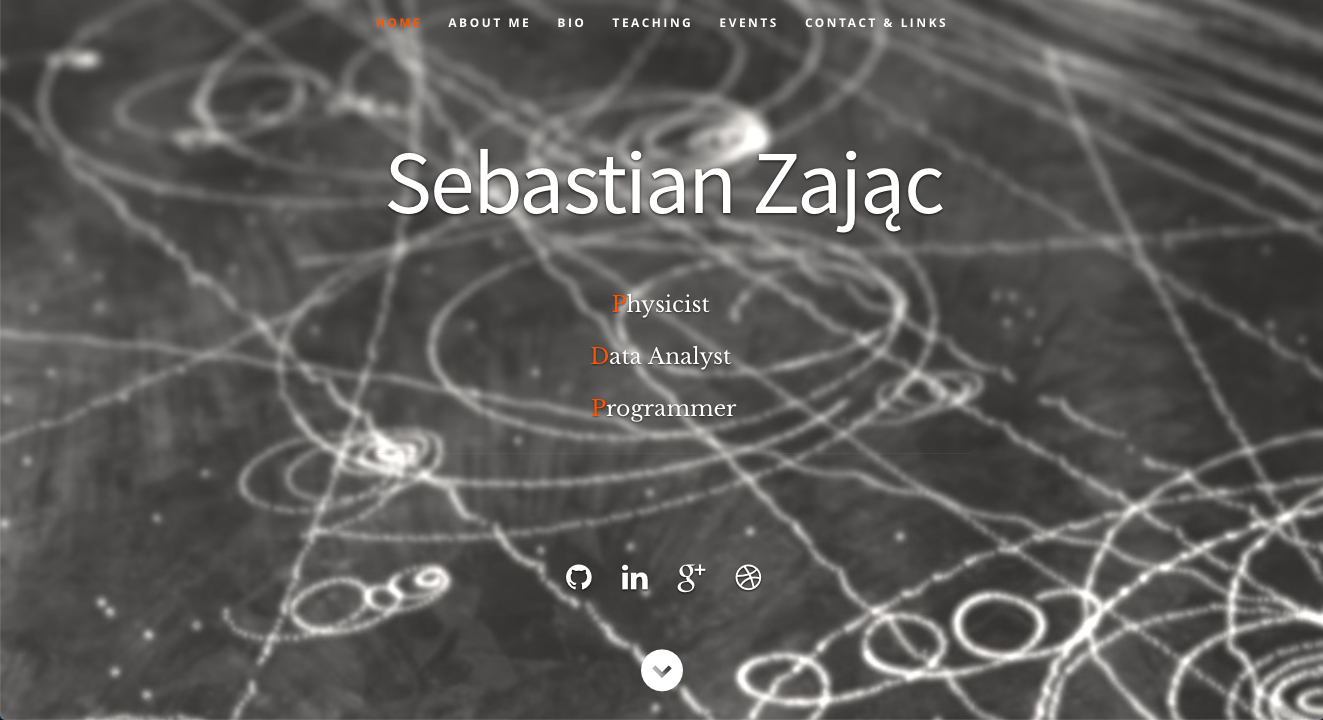
\includegraphics[width=\textwidth]{rys1}
\begin{center}
https://sebastianzajac.pl
\end{center}
\end{frame}

\begin{frame}{Education}
\begin{block}{na początku było ... "Ekono co ? " }
\begin{itemize}
\item 2002-2005 Licencjat - Modelowanie szeregów czasowych za pomocą procesów ARMA i ARIMA.
\item  2005-2007 Mgr - Topologiczne i geometryczne metody w klasycznej i kwantowej teorii pola.
\end{itemize}
\end{block}
\begin{block}{"NoStat"}
chaos $\to$ statystyka $\to$ chaos deterministyczny\\
chaos liczbowy $\to$ teoria mnogości $\to$ teoria kategorii\\
chaos $\to$ statystyka $\to$ mechanika kwantowa $\to$ QFT \\

\end{block}
\begin{center}
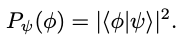
\includegraphics[scale=0.5]{rys2}
\end{center}
\end{frame}

\begin{frame}{ciekawa literatura QM i Statystyka}
\begin{itemize}
\item A. Einstein, B. Podolsky, N. Rosen. "Can Quantum-Mechanical Description of Physical Reality Be Considered Complete? " Physical Review 47 (1935) 777-780.
\item G. Birkhoff, J von Neumann,  “The Logic of Quantum Mechanics”, J. Ann. of Math., 37, 823 (1936).
\item J. Bell "On the Einstein Podolsky Rosen Paradox" Physics 1.3 (1964) 
\item  Aspect, Alain (1976). "Proposed experiment to test the nonseparability of quantum mechanics". Physical Review D. 14 (8): 1944–1951.
\item P. Billingsley "Probability and Measure" NY: John Wiley \& Sons, Inc. 1979
\item Benjamin Feintzeig - Hidden Variables and Commutativity in Quantum Mechanics (2013)
\end{itemize}
\end{frame}


% publikacja Informacja Fishera
\begin{frame}{PHD ...}
\begin{center}
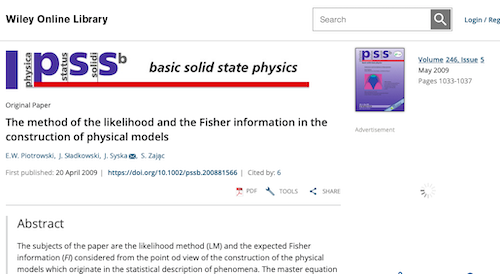
\includegraphics[scale=0.5]{pub4}

"The method of the likelihood and the Fisher information in the construction of physical models." 

{ \tiny E. W. Piotrowski, J. Sładkowski, J.Syska, S.Z. Physica Status Solidi B vol. 246 no. 5 (5.2009).}
\end{center}
\end{frame}

\begin{frame}{PHD - Fizyka}
\begin{block}{Rozprawa doktorska}
"Oscylacje akceleratorowych neutrin z uwzględnieniem ich niestandardowych oddziaływań" Prof. dr hab. Marek Zrałek.

{\tiny „We can’t solve problems by using the same kind of thinking we used when we created them.” (Albert Einstein)}
\end{block}
\includegraphics[scale=0.4]{sm}
\includegraphics[scale=0.05]{feydiag}

\end{frame}

\begin{frame}{Fizyka do dziś...}
\begin{itemize}
\item Jak na podstawie modeli niestatystycznych wybrać, który model realizuje dane i które rozszerzenie jest istotne ? 
\item 7 publikacji dotyczących fizyki neutrin - oddziaływania i zastosowanie dyskretnych grup symetrii do mas i mieszania leptonów. 
\item udział w 2 grantach, prezentacje na 5 międzynarodowych konferencjach neutrinowych. 
\end{itemize}
\begin{center}
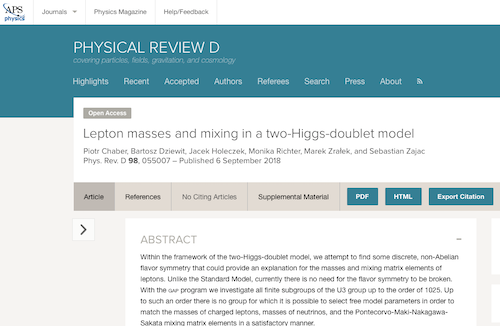
\includegraphics[scale=0.3]{pub3}
\end{center}
\end{frame}



\begin{frame}{Poza Fizyką .... ale z fizykami na UW}
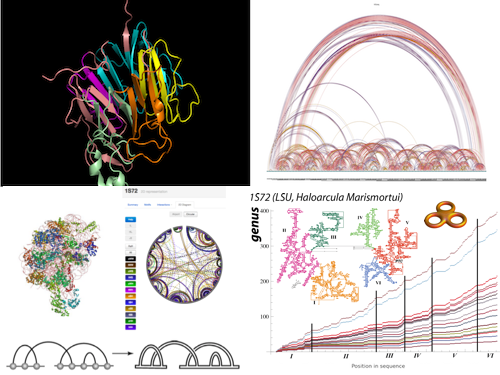
\includegraphics[width=\textwidth]{protein.png}
\end{frame}

% slajd 2 Fizyka
\frame{\frametitle{Gdzie znajdziesz diagramy chordowe ? }
\begin{block}{Physics}
\begin{center}
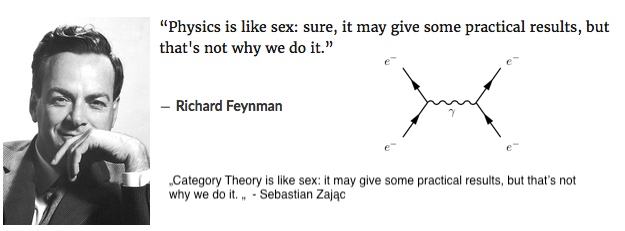
\includegraphics[scale=0.5]{richard.png}
\end{center}
\end{block}
\begin{block}{Server danych}
http://genus.fuw.pl
\end{block}
}


\begin{frame}
\begin{center}
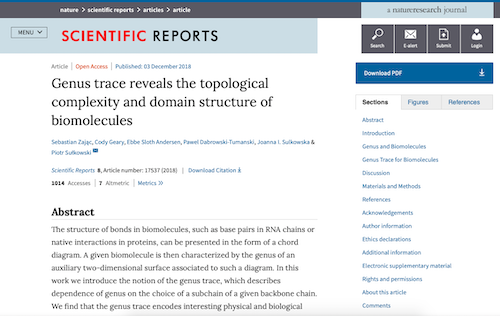
\includegraphics[scale=0.6]{pub1}
\end{center}
\end{frame}


\begin{frame}
\begin{center}
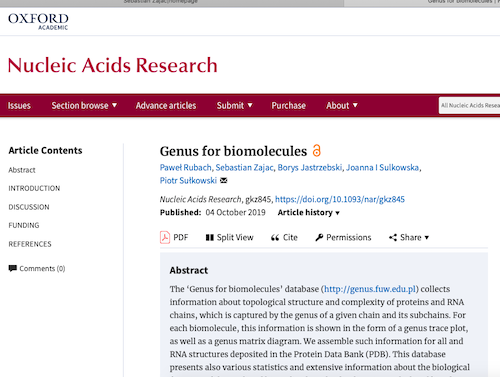
\includegraphics[scale=0.6]{pub2}
\end{center}
\end{frame}

\begin{frame}{Poza Fizyką .... ale z matematykami z UKSW}
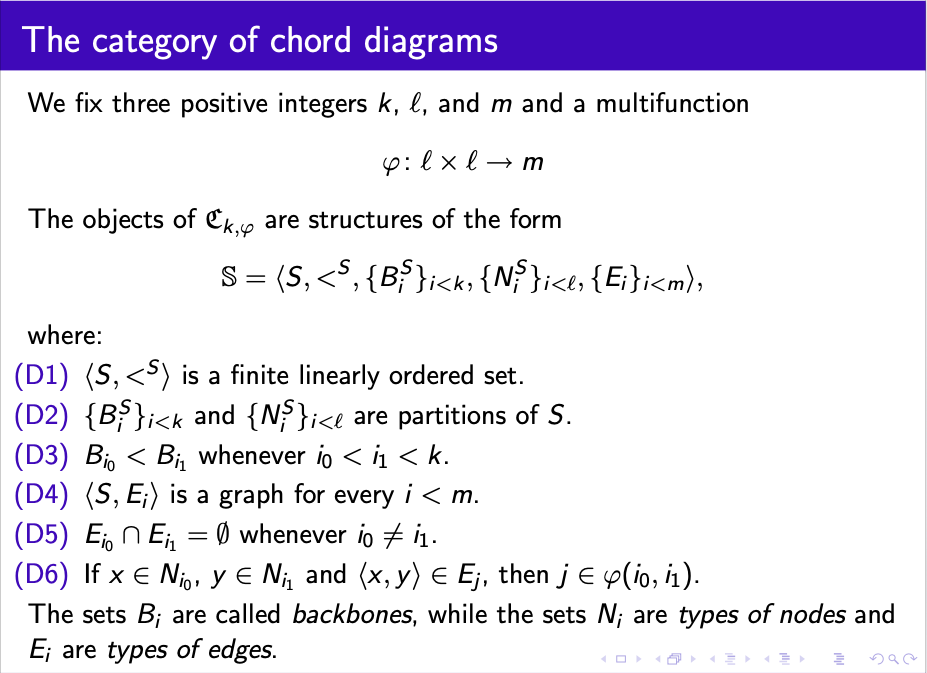
\includegraphics[scale=0.35]{zd1}
\end{frame}

\begin{frame}{Poza Fizyką .... ale z matematykami z UKSW}
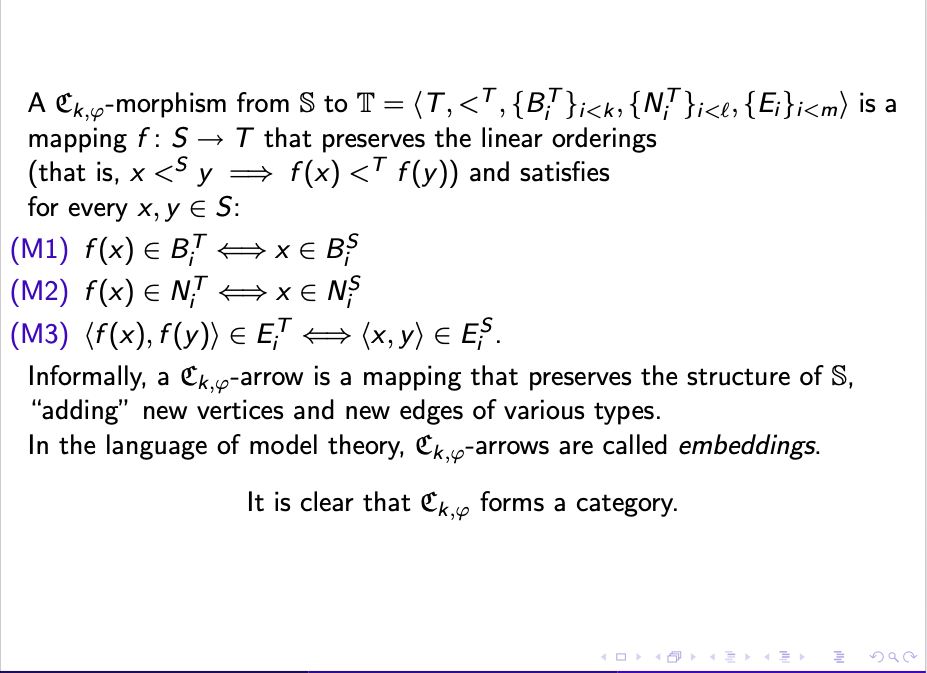
\includegraphics[scale=0.35]{zd2}
\end{frame}

\begin{frame}{Na SGH i w biznesie}

\begin{itemize}
\item Nowy przedmiot dla studentów SGH - Analizy danych w czasie rzeczywistym.
\item Twórca portalu do analiz plików JPK
\item Współtwórca darmowej i płatnej wersji biblioteki w pythonie do automatycznego generowania modeli scoringowych - Advanced Scorecard Builder.
\item Programowanie i przetwarzanie danych oraz statystyka w SAS. 
\item Badania statutowe - Metody doboru zmiennych z wykorzystaniem narzędziami machine i deep learning.
\end{itemize}
\end{frame}
\begin{frame}{SGH wydarzenia}
\begin{itemize}
\item 28.XI.2019 Konferencja - Analityka dla Biznesu
\item 4.XII.2019 roku w Sali 2b w budynku C , odbędzie się promocja książki {\bf Modelowanie dla biznesu}.\\ {\tiny  https://businessintelligence.pl/pl/wizualizacja-wynikow-modelowania-z-qlik-sense/  }
\end{itemize}
\begin{center}

\includegraphics[scale=0.1]{book} 
\end{center}
\end{frame}


\begin{frame}{Poza Światem}

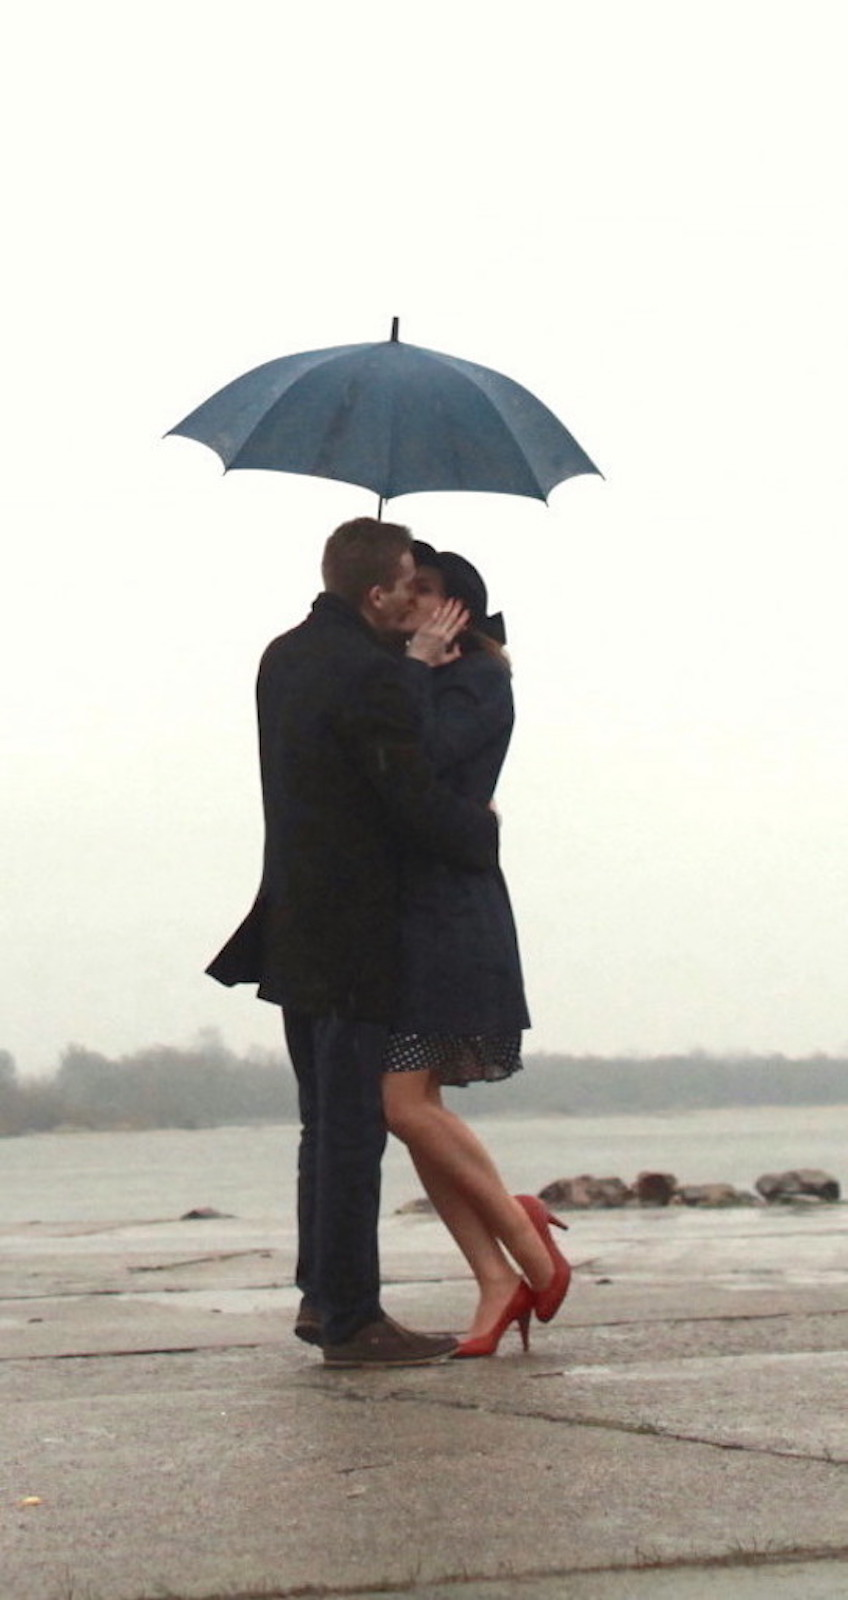
\includegraphics[scale=0.1]{parasol} 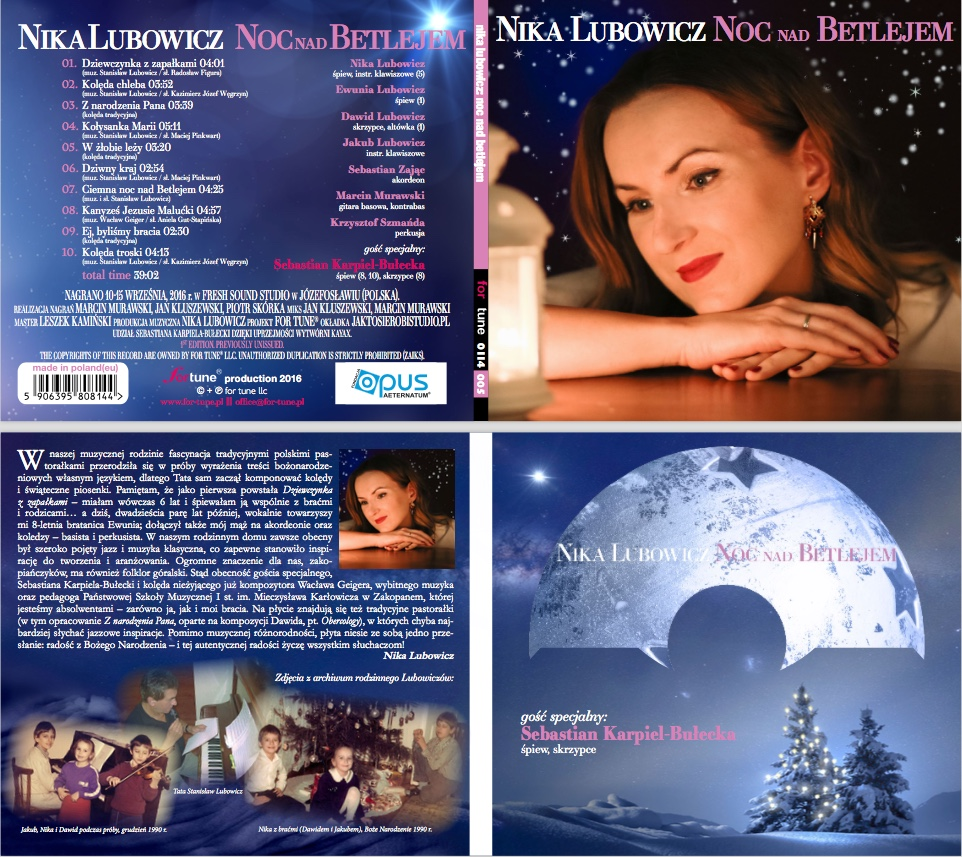
\includegraphics[scale=0.2]{plyta}
\end{frame}

\begin{frame}{}
\begin{block}{Wyjaśnienie}
 "NoSTAT" czytamy i tłumaczymy jako {\bf Not Only Stat} !  
\end{block}
\begin{block}{}
\begin{center}
Dziękuję za uwagę !
\end{center}
\end{block}
\end{frame}


\end{document}
